\chapter{Considerações Finais}

O desenvolvimento do sistema web para controle de estoque e vendas da loja \textbf{Tropical Mix} representa uma iniciativa relevante na aplicação prática dos conhecimentos adquiridos ao longo do curso, aliando teoria e experiência profissional em um contexto real de gestão empresarial. O projeto cumpriu o propósito de propor uma solução tecnológica acessível e de baixo custo, voltada para a digitalização de processos internos em pequenos negócios, um desafio ainda presente em grande parte das microempresas brasileiras.

Ao longo do projeto, a equipe pôde vivenciar todas as etapas do ciclo de desenvolvimento de software, desde o planejamento e análise de requisitos até a implementação e documentação técnica. A utilização de metodologias ágeis, aliadas a ferramentas colaborativas como GitHub, Overleaf e Notion, contribuiu para a organização das tarefas e o acompanhamento contínuo das entregas, assegurando uma gestão eficiente do trabalho em equipe. O emprego de tecnologias amplamente reconhecidas no mercado, como \textit{React}, \textit{Flask} e \textit{MySQL}, reforçou o compromisso do grupo em desenvolver uma solução moderna, funcional e alinhada às práticas profissionais.

Espera-se que o sistema desenvolvido contribua para otimizar o controle operacional da \textbf{Tropical Mix}, oferecendo maior agilidade, precisão e transparência na gestão de produtos e vendas. Além de seu valor técnico, o projeto reafirma o papel social e formativo da extensão universitária, que aproxima a comunidade acadêmica das demandas reais da sociedade, promovendo aprendizado significativo e impacto positivo.

\section{Dificuldades, Escolhas e Descartes}

O desenvolvimento do projeto apresentou desafios importantes, que contribuíram diretamente para o amadurecimento técnico e organizacional da equipe. A principal dificuldade enfrentada foi a curva de aprendizado associada às tecnologias escolhidas, que exigiu pesquisa constante, prática intensiva e integração entre os membros para superação de barreiras técnicas e conceituais.

Além desse fator, destacaram-se outras dificuldades enfrentadas ao longo do processo, sintetizadas na Tabela~\ref{fig:dificuldades}.

\begin{figure}[H]
  \centering
  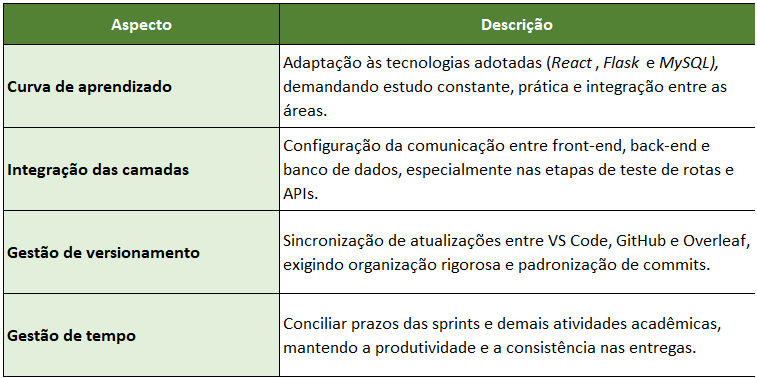
\includegraphics[width=0.9\textwidth]{documentacao/LaTex/Capítulos/img/Conclusão/dificuldades.png}
  \caption{Tabela de Dificuldades do Projeto}
  \fonte{Elaborado pelos autores.}
  \label{fig:dificuldades}
\end{figure}

Nas decisões técnicas, optou-se por priorizar ferramentas gratuitas, amplamente utilizadas e com documentação acessível, garantindo a viabilidade do projeto mesmo sem orçamento destinado à sua execução. O \textit{Flask} foi escolhido pela leveza e compatibilidade com o modelo de API proposto, o \textit{React} pela flexibilidade na criação de interfaces dinâmicas e o \textit{MySQL} por sua confiabilidade e ampla adoção no mercado.

Durante o desenvolvimento, também ocorreram descartes estratégicos, como a exclusão da camada de interface voltada ao cliente final, mantendo o foco da aplicação na gestão interna da loja. Essa escolha permitiu reduzir a complexidade do sistema e garantir a conclusão das funcionalidades essenciais dentro do prazo estabelecido.

Em síntese, o projeto proporcionou um aprendizado abrangente, tanto técnico quanto colaborativo. A experiência reforçou a importância da comunicação constante, do planejamento estruturado e da aplicação de metodologias ágeis no contexto acadêmico. Mais do que um produto tecnológico, o sistema desenvolvido representa um exercício de integração, comprometimento e crescimento coletivo, reafirmando o potencial transformador da tecnologia quando aplicada a contextos reais e acessíveis.
